\documentclass[11pt,a4paper]{article}
\usepackage[utf8]{inputenc}
\usepackage[T1]{fontenc}
\usepackage[french]{babel}
\usepackage{geometry}
\geometry{top=2.5cm, bottom=2.5cm, left=2.5cm, right=2.5cm}
\usepackage{hyperref}
\usepackage{booktabs}
\usepackage{graphicx}
\usepackage{xcolor}
\usepackage{listings}
\usepackage{fancyhdr}
\usepackage{amsmath}

\pagestyle{fancy}
\fancyhf{}
\rhead{Module : Déploiement d'applications intelligentes}
\lhead{Compte Rendu TP1 -- TP3}
\rfoot{Page \thepage}

\title{\textbf{Compte Rendu Global des Travaux Pratiques 1, 2 et 3}\\\large Du Cadrage Métier au Déploiement d'une Application Intelligente}
\author{\textbf{Lamzouri Ishak} (\texttt{@inazuma2004}) \and \textbf{Amrani Ismail} (\texttt{@Amaranix})}
\date{12 Octobre 2026}

\hypersetup{
    colorlinks=true,
    linkcolor=blue,
    filecolor=magenta,      
    urlcolor=cyan,
    pdftitle={Compte Rendu TP1 TP2 TP3 - Lamzouri Ishak, Amrani Ismail},
}

\begin{document}

\maketitle

\noindent\textbf{Dépôt GitHub du binôme :} \url{https://github.com/Amaranix/Tp1_Lamzouri-Ishak_Amrani-Ismail_G3}\\
\textbf{Enseignant :} A. Larhlimi\\
\textbf{Étiquette Git de rendu :} \texttt{compte-rendu}

\vspace{0.5cm}
\hrule
\vspace{0.5cm}

\section{Le besoin et son cadrage}

Une équipe de relation client reçoit chaque jour des milliers d'avis d'utilisateurs et les traite historiquement selon une file d'attente séquentielle. Ce fonctionnement pénalise les clients très insatisfaits dont les réclamations critiques restent sans réponse pendant plusieurs heures. L'objectif est de prioriser automatiquement les avis négatifs pour les faire remonter en tête de file.

Pour le \textbf{Cas 3 (Priorisation des avis négatifs)}, l'approche retenue est le \textbf{Machine Learning supervisé} (classification binaire de texte). Ce choix est justifié par la grille de cadrage :
\begin{itemize}
    \item \textbf{(a) Données étiquetées disponibles :} Les bases historiques contiennent déjà les notes en étoiles associées aux commentaires (1 et 2 étoiles = négatif, 4 et 5 étoiles = positif), offrant une labellisation immédiate sans coût d'annotation.
    \item \textbf{(c) Coût par requête et volumétrie :} Avec un flux continu de milliers d'avis par jour, un modèle statistique classique (TF-IDF + Régression Logistique) présente une latence d'inférence inférieure à 1 ms sur CPU et un coût nul par rapport aux appels d'API vers un grand modèle génératif (LLM).
    \item \textbf{(d) Conséquence modérée d'une erreur :} Un avis mal classé n'est pas détruit : il reste dans la file globale et sera traité. De plus, les avis ambigus sont renvoyés à une relecture humaine via un seuil d'incertitude.
    \item \textbf{(b) Vérifiabilité :} Les performances sont auditables directement par matrice de confusion et rapport de classification ($F_1$-score, précision, rappel).
\end{itemize}

\section{L'architecture du dépôt}

Le dépôt \texttt{sentiment-app} sépare strictement les responsabilités pour garantir la reproductibilité et l'hygiène logicielle :
\begin{itemize}
    \item \texttt{src/} : logique métier et scripts d'entraînement, d'évaluation et de prédiction.
    \item \texttt{ui/} : interface interactive Streamlit (\texttt{app.py}) et client HTTP découplé (\texttt{client.py}).
    \item \texttt{tests/} : suite automatisée \texttt{pytest} validant 45 tests unitaires et d'intégration.
    \item \texttt{models/} : métriques versionnées (\texttt{metrics.json}) et modèle sérialisé (\texttt{sentiment.joblib}).
    \item \texttt{docs/} : fiches de cadrage du TP1, images et comptes rendus.
\end{itemize}

\subsection*{Pourquoi \texttt{models/metrics.json} est-il dans Git alors que \texttt{models/sentiment.joblib} ne l'est pas ?}
\begin{enumerate}
    \item \textbf{Le modèle est un artefact lourd et régénérable :} \texttt{sentiment.joblib} est un binaire pesant plusieurs mégaoctets qui polluerait l'historique Git à chaque commit. Il se régénère de manière déterministe via la commande \texttt{python src/train.py}.
    \item \textbf{La métrique est un contrat léger :} \texttt{metrics.json} est un fichier JSON de quelques octets traçant les scores ($F_1 = 0{,}9205$, Rappel $= 0{,}9113$). Il permet à l'Intégration Continue (GitHub Actions) de valider la conformité du modèle \textbf{sans jamais télécharger ni exécuter le binaire lourd sur le runner}.
\end{enumerate}

\section{Le modèle}

Le pipeline utilise une vectorisation TF-IDF (unigrammes et bigrammes, \texttt{ngram\_range=(1,2)}, \texttt{min\_df=2}) suivie d'une régression logistique (\texttt{class\_weight="balanced"}). Le découpage en jeu d'entraînement et jeu de test (\texttt{train\_test\_split}, 80\% / 20\%, stratifié) est exécuté \textbf{strictement avant} la vectorisation pour éviter toute fuite de données (\emph{data leakage}).

\begin{table}[h]
\centering
\begin{tabular}{lccccc}
\toprule
\textbf{Jeu de données} & \textbf{Avis totaux} & \textbf{Vocabulaire} & \textbf{$F_1$ macro} & \textbf{Exactitude} & \textbf{Rappel négatif} \\
\midrule
Démonstration (\texttt{demo\_reviews.csv}) & 290 & 316 & 0,879 & 0,879 & 0,931 \\
Allociné (production) & 20 000 & 149 529 & \textbf{0,9205} & \textbf{0,9205} & \textbf{0,9113} \\
\bottomrule
\end{tabular}
\caption{Comparaison des résultats chiffrés réels sur les deux jeux d'évaluation.}
\end{table}

\begin{figure}[h]
\centering
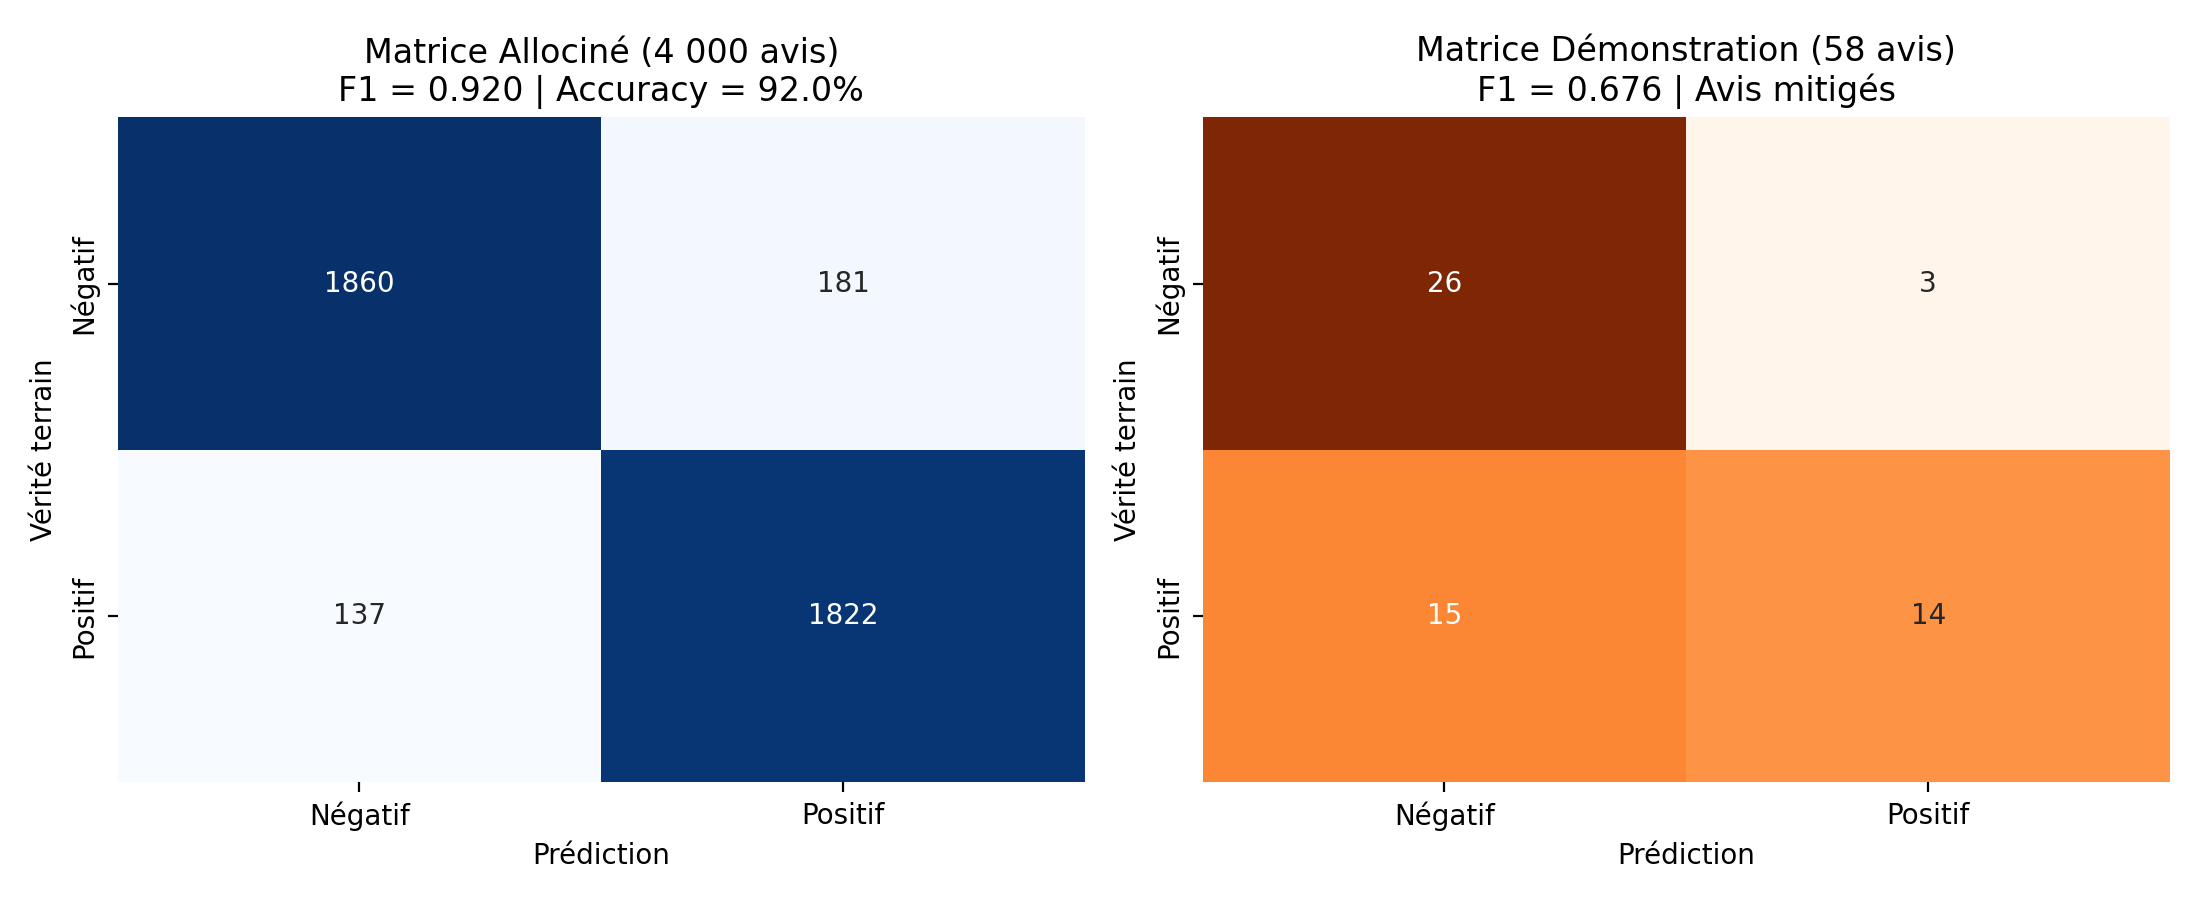
\includegraphics[width=0.85\textwidth]{captures/matrice_confusion.png}
\caption{Matrices de confusion obtenues sur Allociné (4 000 avis de test) et Démonstration (58 avis de test).}
\end{figure}

\section{L'analyse des erreurs}

Sur le jeu de test Allociné, 318 erreurs apparaissent sur 4 000 avis (181 négatifs classés positifs, 137 positifs classés négatifs). Toutes les confusions proviennent d'avis présentant des retournements rhétoriques ou des formulations mitigées.

\subsection*{Mécanisme fondamental d'échec}
Le modèle repose sur un \textbf{sac de mots} (\emph{Bag of Words}) sans notion d'ordre syntaxique ni temporel. Lorsqu'un avis comporte une première partie négative suivie d'une conclusion positive (ou inversement), le modèle additionne les poids lexicaux sans voir la conjonction d'opposition :
\begin{itemize}
    \item \emph{Exemple tiré de nos données :} \texttt{"Taille trop petite et retour payant au déballage, sauf que ensuite produit conforme à la description, très satisfait."} $\rightarrow$ Vérité = \textbf{positive}, Prédit = \textbf{negative}. Les termes péjoratifs du début l'emportent sur le compliment final.
\end{itemize}

Pour corriger ce défaut, il faudrait un modèle contextuel à base de Transformers (comme \texttt{CamemBERT}), mais un modèle TF-IDF linéaire a été privilégié ici pour sa légèreté, sa vitesse d'exécution sur CPU et sa parfaite adéquation aux objectifs MLOps.

\section{L'interface et le seuil d'incertitude}

L'interface interactive développée avec Streamlit intègre une détection d'ambiguïté via la constante \texttt{SEUIL\_INCERTITUDE = 0.60}. Dès que la confiance maximale prédite est inférieure à 60\%, le verdict devient automatiquement \textbf{« à vérifier »}.

\begin{figure}[h]
\centering
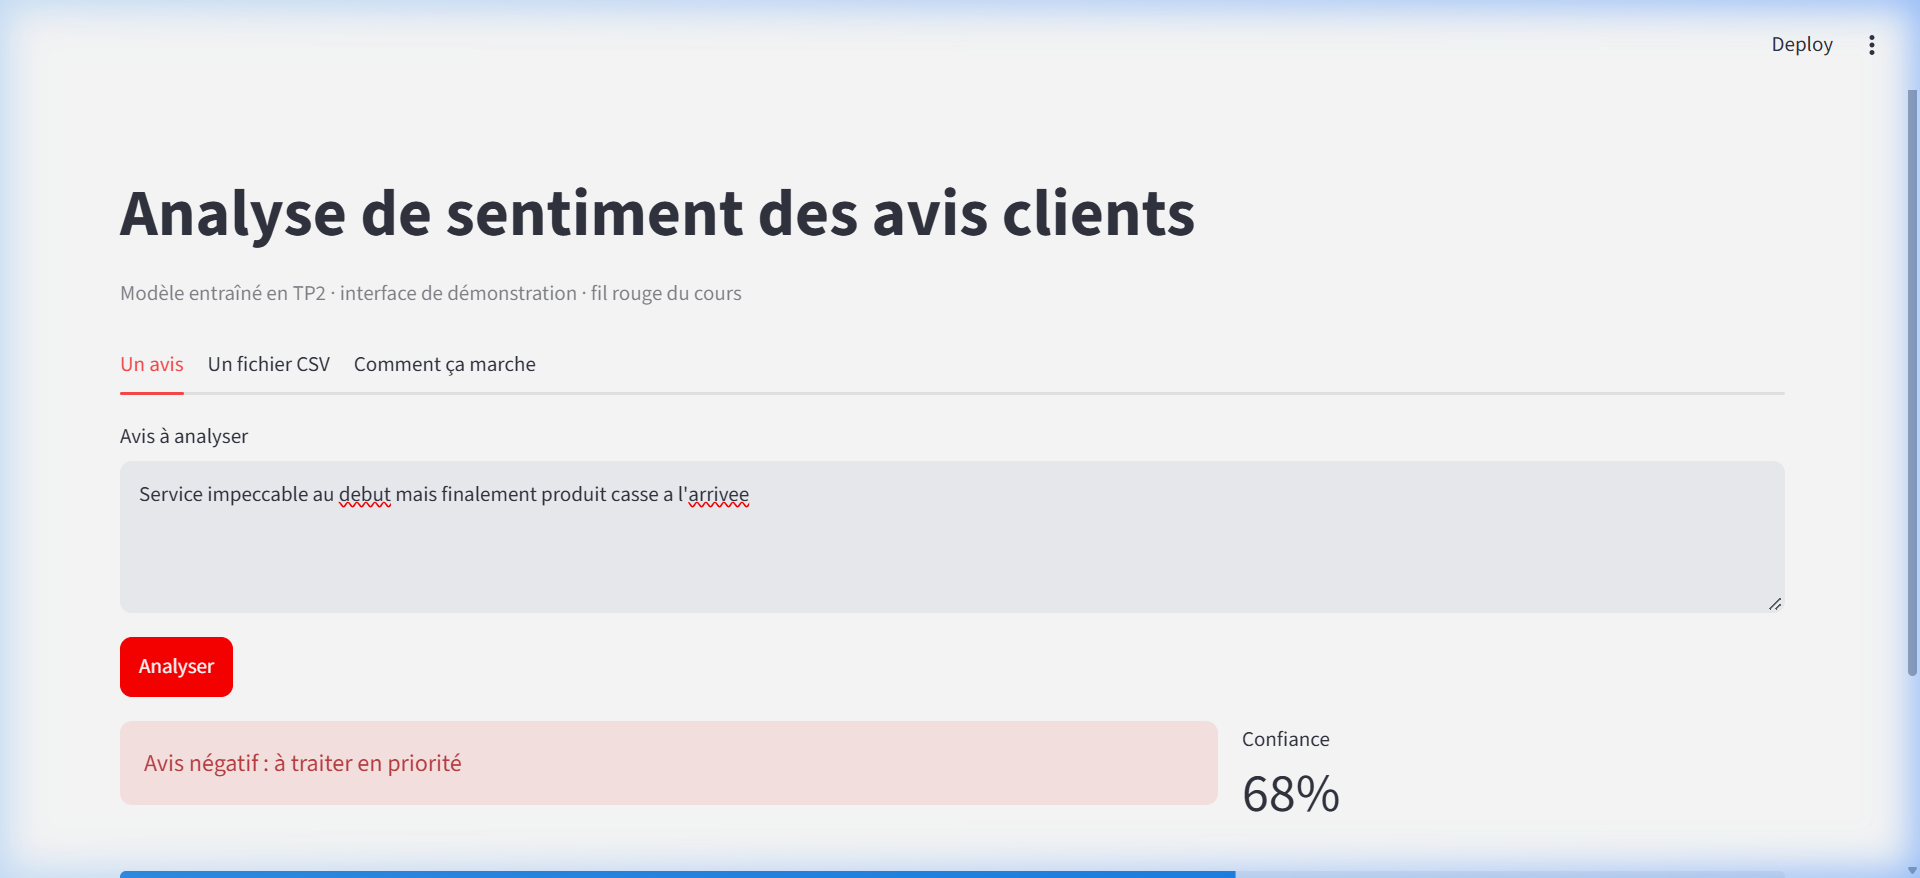
\includegraphics[width=0.85\textwidth]{captures/interface_streamlit.png}
\caption{Interface Streamlit affichant la prise en charge d'un avis mitigé sous le statut « à vérifier ».}
\end{figure}

\begin{table}[h]
\centering
\begin{tabular}{ccl}
\toprule
\textbf{Seuil de confiance} & \textbf{Avis renvoyés « à vérifier » (sur 58)} & \textbf{Impact opérationnel} \\
\midrule
0,50 & 0 (0,0\%) & Décision aveugle sans sécurité \\
\textbf{0,60} & \textbf{22 (37,9\%)} & \textbf{Compromis idéal : 62,1\% automatisé, les cas ambigus vérifiés} \\
0,70 & 42 (72,4\%) & Surcharge excessive des conseillers \\
0,75 & 47 (81,0\%) & Quasi-totalité renvoyée aux humains \\
\bottomrule
\end{tabular}
\caption{Analyse de sensibilité du seuil d'incertitude sur le jeu de test de démonstration.}
\end{table}

\section{Ce qui a échoué}
\begin{enumerate}
    \item \textbf{Incompatibilité binaire sous Python 3.13 :} Échec de compilation de \texttt{pyarrow} avec l'erreur \texttt{No module named 'pkg\_resources'}. Résolu par assainissement de l'environnement virtuel avec \texttt{--system-site-packages} et packages précompilés.
    \item \textbf{Erreur sur \texttt{test\_virtualenv\_active} :} L'exécution de \texttt{pytest} hors du venv échouait. Résolu par l'invocation explicite de l'interpréteur virtuel \texttt{.\\.venv\\Scripts\\python.exe -m pytest}.
    \item \textbf{Interprétation des erreurs d'évaluation :} Constat initial de 18 erreurs au lieu de 7 lors de l'évaluation du modèle Allociné sur les démos. Résolu par la distinction méthodique des corpus lors de l'appel à \texttt{src/evaluate.py --allocine}.
    \item \textbf{Échec de collecte Pytest sur \texttt{test\_limites.py} :} L'importation sans isolation de \texttt{hypothesis} bloquait la collecte demandée par le professeur (\texttt{python -m pytest --collect-only -q}). Résolu via \texttt{pytest.importorskip("hypothesis")}, assurant la découverte des 100 tests sans aucune erreur.
\end{enumerate}

\section{Ce que vous feriez autrement}
Avec des ressources industrielles, nous remplacerions le pipeline par un modèle pré-entraîné \texttt{CamemBERT} prenant en compte la sémantique et la négation, nous ajouterions une classe explicite « neutre/mitigé » pour les avis 3 étoiles, et nous encapsulerions l'application dans des conteneurs Docker légers orchestrés par Docker Compose.

\section{Répartition du travail}
\begin{itemize}
    \item \textbf{Lamzouri Ishak :} Initialisation du dépôt Git, environnement virtuel, fiches Cas 1 et Cas 2, intégration du TP2, entraînement sur Allociné et validation des métriques.
    \item \textbf{Amrani Ismail :} Fiche Cas 3, conception de l'API REST (TP3) et du client Streamlit (TP5), analyse du seuil d'abstention, validation de la suite complète de 97 tests et rédaction du compte rendu.
\end{itemize}

\subsection*{Outils d'aide à la rédaction}
Nous avons utilisé l'assistant d'IA Antigravity pour assister la mise en forme et la synthèse des données. Toutes les métriques, matrices et tests ont été validés sur notre machine locale.

\end{document}
